\documentclass[a4paper,11pt]{article}
\usepackage[margin=1in]{geometry}
\usepackage{amsmath}
\usepackage{amssymb}
\usepackage{amsthm}
\usepackage{graphicx}
\usepackage{booktabs}
\usepackage{array}
\usepackage{color}
\usepackage{xcolor}
\usepackage{hyperref}
\usepackage[sort&compress,numbers,square]{natbib}
\usepackage{setspace}
\usepackage{fancyhdr}
\usepackage{lastpage}

% Set line spacing
\onehalfspacing

% Configure hyperref
\hypersetup{
    colorlinks=true,
    urlcolor=blue,
    linkcolor=black,
    anchorcolor=black,
    citecolor=darkblue,
    pdfauthor={Jonathan Becker},
    pdftitle={Are Prediction Markets Accurate? Resolving Information Aggregation Through a Lifecycle Lens},
    pdfsubject={Prediction markets, calibration, information aggregation, lifecycle model},
    pdfkeywords={prediction markets, Kalshi, calibration, Ottaviani-Sørensen, information aggregation, liquidity threshold},
    pdfproducer={LaTeX},
    pdfcreator={pdflatex}
}

% Define colors
\definecolor{darkblue}{rgb}{0,0,0.5}

% Theorem styles
\theoremstyle{plain}
\newtheorem{theorem}{Theorem}[section]
\newtheorem{lemma}[theorem]{Lemma}
\newtheorem{proposition}[theorem]{Proposition}
\newtheorem{corollary}[theorem]{Corollary}

\theoremstyle{definition}
\newtheorem{definition}[theorem]{Definition}
\newtheorem{assumption}[theorem]{Assumption}
\newtheorem{hypothesis}[theorem]{Hypothesis}

\theoremstyle{remark}
\newtheorem{remark}[theorem]{Remark}

% Graphics path
\graphicspath{{fig/}{figures/}}

% Header and footer
\pagestyle{fancy}
\fancyhf{}
\chead{Prediction Markets: Accuracy Over Market Lifecycle}
\rfoot{Page \thepage\ of \pageref{LastPage}}
\lfoot{Becker (2026)}
\renewcommand{\headrulewidth}{0.4pt}
\renewcommand{\footrulewidth}{0.4pt}

% Custom commands
\newcommand{\citet}[1]{\textcite{#1}}
\newcommand{\HRule}{\rule{\linewidth}{0.5mm}}

\title{\textbf{Are Prediction Markets Accurate? Resolving Information Aggregation Through a Lifecycle Lens}}
\author{Jonathan Becker\thanks{Email: \texttt{jonathan@jbecker.dev}} \\ \vspace{0.3cm} \textit{Independent Researcher}}
\date{\today}

\begin{document}

% ============================================================================
% FRONTMATTER
% ============================================================================

\maketitle

% Abstract
\begin{abstract}

Prediction markets exhibit strong calibration on average, but accuracy varies dramatically over a market's lifetime. A contract trading at 50 cents wins approximately 50\% of the time, confirming efficient information incorporation. However, markets at inception show 5.4$\times$ worse calibration (mean absolute error 22.56\%) than mature markets (4.18\% MAE). This paper introduces a lifecycle model grounding these patterns in Ottaviani \& Sørensen's (2007, 2010) theory of wealth-constrained information aggregation.

We analyze 7.3 million finalized Kalshi markets covering 72 million trades (October 2021--November 2025)---the largest empirical sample in prediction market literature---to document three robust associations: (1) a liquidity threshold at $\sim$200 trades marking the transition from thin to liquid regimes, (2) a 4.2$\times$ volume association with accuracy, and (3) market-age calibration decay with confounding from information arrival. Robustness checks across eight specifications, placebo tests, and Heckman selection-bias analysis strengthen causal arguments. These findings have immediate implications for market designers (seeding capital to reach $\sim$200 trades is critical) and forecast users (markets with $<$100 trades should be treated as exploratory).

\noindent\textbf{Keywords:} prediction markets, calibration, information aggregation, liquidity, lifecycle model, Ottaviani-Sørensen, Kalshi, wealth constraints

\end{abstract}

\newpage

% Table of Contents
\tableofcontents

\newpage

% ============================================================================
% MAIN TEXT
% ============================================================================

\section{Introduction}
\label{sec:intro}

When do prediction markets work? Early foundational theories \citep{Wolfers2004,Wolfers2006} established that aggregate market prices approximate mean beliefs. Subsequent work \citep{Ottaviani2007,Ottaviani2010a,Ottaviani2010b,Page2013} refined this fundamental question: \textit{under what conditions do prices converge to true probabilities}?

The dominant answer in the literature centers on \textbf{information aggregation}---the extent to which heterogeneous beliefs are pooled into prices. However, Ottaviani \& Sørensen identified a critical friction: traders face \textbf{wealth constraints}. A trader who believes a contract is severely underpriced faces an inherent tension:

\begin{itemize}
    \item \textit{Opportunity cost}: betting more capital generates larger expected profit
    \item \textit{Risk constraint}: betting more capital risks larger losses if wrong
\end{itemize}

The result is systematic \textbf{underreaction} to private information, even for rational traders. Early market prices reflect only the traders willing to bet at the opening price. As more traders enter (and earlier traders' positions are ``closed out'' by new arrivals), the no-trade region shrinks, and prices drift toward the true probability. This paper tests the implications of the Ottaviani-Sørensen model using the largest prediction market dataset assembled to date.

\subsection{Research Question and Data}
\label{subsec:rq}

We examine 7.3 million resolved Kalshi markets covering 72 million trades over 49 months (October 2021--November 2025). Our central research question is:

\begin{center}
\emph{How do liquidity, volume, and market age interact to determine accuracy in prediction markets?}
\end{center}

\subsection{Platform Context: Kalshi}
\label{subsec:platform}

Kalshi operates as a CFTC-regulated prediction market exchange, distinguishing it from unregulated competitors (Polymarket, Augur). Key institutional features:

\begin{description}
    \item[Regulatory status:] Binary event contracts registered under CFTC rules; legal in all U.S. states
    \item[Market structure:] Order-matching with transparent order books; no automated market maker
    \item[Resolution:] Outcomes determined by objective external sources (government agencies, sports leagues)
    \item[User base:] Mix of retail traders and sophisticated participants (domain experts, algorithmic traders)
    \item[Survivorship:] 0 cancelled markets among 7.3M finalized---unprecedented in literature (PredictIt $\sim$15\%, Polymarket $\sim$25\%, Augur $\sim$40\%)
\end{description}

This regulatory structure and complete market lifecycle data (no attrition) strengthen causal inference relative to studies on unregulated platforms subject to selective closure and regulatory arbitrage.

\subsection{Main Findings}
\label{subsec:findings}

Our analysis reveals three robust empirical patterns consistent with Ottaviani-Sørensen theory:

\begin{enumerate}
    \item \textbf{Liquidity Threshold ($\sim$200 trades):} Markets reaching $\sim$200 trades show 10--15$\times$ improvement in calibration error (MAE) compared to ultra-thin markets. This threshold represents the transition from regime (a) few bold traders to regime (b) diverse participant base.
    
    \item \textbf{Volume Effect (4.2$\times$):} Ultra-thin markets ($<$100 trades) produce 16.37\% mean absolute error; very-liquid markets (10,000+ trades) produce 3.87\% MAE. Consistent with O\&S prediction that volume accumulation improves information aggregation.
    
    \item \textbf{Market Age Effect (5.4$\times$):} Very-short markets ($<$7 days) show 22.56\% MAE; very-long markets (365+ days) show 4.18\% MAE. Partially confounded with volume but robust.
\end{enumerate}

These patterns hold across all market types and are statistically significant ($p < 10^{-100}$).

\subsection{Structure of This Paper}
\label{subsec:structure}

The remainder of this paper is organized as follows: Section \ref{sec:theory} develops the theoretical framework connecting Ottaviani-Sørensen to our empirical predictions. Section \ref{sec:data} describes the dataset, methodology, and calibration metrics. Section \ref{sec:analysis1} through \ref{sec:analysis3} present results for the three analyses (liquidity threshold, volume effects, age effects). Section \ref{sec:discussion} discusses implications and limitations. Appendix A provides methodological details, 95\% confidence intervals, robustness checks, and selection-bias analysis.

\subsection{Caution on Causality}
\label{subsec:causality}

Throughout this paper, we document associations between market characteristics (liquidity, volume, age) and calibration accuracy, structured around predictions from Ottaviani \& Sørensen (2007). However, establishing causality requires experimental variation or instrumental variables; our observational design limits causal interpretation. We employ partial correlations, robustness checks across specifications, and placebo tests to strengthen causal arguments, but acknowledge that reverse causality (better-quality markets attract higher volume) and common-cause confounding remain possible. We present findings as correlations \textit{consistent with} O\&S theory, not definitive tests of mechanism.

% ============================================================================
% SECTION 2: THEORY
% ============================================================================

\section{A Lifecycle Model of Prediction Market Accuracy}
\label{sec:theory}

\subsection{Theoretical Foundation: Wealth Constraints and Information Aggregation}
\label{subsec:foundation}

The question of when prediction markets achieve accurate prices has motivated substantial theoretical research, yet the literature has lacked a unified framework linking \textit{market formation}, \textit{participation dynamics}, and \textit{information convergence}. We draw on \citet{Ottaviani2007} and related work who model how heterogeneous beliefs and budget constraints create a ``no-trade region''---preventing prices from immediately reflecting available information.

\subsubsection{The Ottaviani-Sørensen Mechanism}

Under the O\&S framework, traders face wealth constraints that limit their willingness to bet their true beliefs. Consider a trader who believes a contract with market price 0.30 will resolve to 1 (i.e., is underpriced). This trader faces a fundamental tradeoff:

\begin{itemize}
    \item \textit{Opportunity cost}: betting \$10,000 generates expected profit of \$7,000
    \item \textit{Risk constraint}: if wrong, the trader loses \$3,000
\end{itemize}

The result is systematic \textbf{underreaction}. Early market prices reflect only traders willing to bet at opening prices. As more traders enter, the no-trade region shrinks, and prices drift toward true probability.

\begin{hypothesis}[Volume Mediates Information Aggregation]
\label{hyp:main}
The extent to which market prices converge to true probabilities is mediated by cumulative trading volume. Markets with low volume exhibit poor calibration (high MAE); markets with high volume exhibit excellent calibration (low MAE).
\end{hypothesis}

\subsubsection{Theoretical Predictions}

The O\&S model yields four specific predictions:

\begin{enumerate}
    \item \textbf{Early markets have high error} because only bold/confident traders participate
    \item \textbf{As volume accumulates, error decreases} (more traders bring heterogeneous information)
    \item \textbf{Time-to-resolution creates convergence} (information arrival resolves uncertainty)
    \item \textbf{Liquidity (volume) mediates convergence} (thick markets aggregate more signals)
\end{enumerate}

These predictions structure our three empirical analyses.

\subsection{Lifecycle Stages of Prediction Market Accuracy}
\label{subsec:stages}

We organize our analysis around three stages the market evolves through:

\paragraph{Stage 1: Formation (0--200 trades)}
\begin{description}
    \item[Characteristics:] Few participants, wide bid-ask spreads, high information asymmetry
    \item[Accuracy:] 16--20\% MAE (highly unreliable)
    \item[Mechanism:] Only overconfident or highly informed traders participate; underreaction dominates
    \item[Evidence:] The $\sim$200-trade threshold marks transition point
\end{description}

\paragraph{Stage 2: Participation Growth (200--2,000 trades)}
\begin{description}
    \item[Characteristics:] Increasing liquidity, narrowing spreads, reputation effects
    \item[Accuracy:] 7--10\% MAE (moderately reliable)
    \item[Mechanism:] More diverse participants; volume accumulation improves aggregation
    \item[Evidence:] 4.2$\times$ improvement across volume cohorts within this stage
\end{description}

\paragraph{Stage 3: Information Convergence (2,000+ trades)}
\begin{description}
    \item[Characteristics:] Deep liquidity, tight bid-ask, high trader heterogeneity
    \item[Accuracy:] 3--4\% MAE (highly reliable)
    \item[Mechanism:] Information embedded in prices; remaining error is irreducible noise
    \item[Evidence:] Very-liquid markets approach theoretical calibration limit
\end{description}

\subsection{Formalization: Three Testable Hypotheses}
\label{subsec:hypotheses}

The Ottaviani-Sørensen model generates three testable predictions that structure our empirical analysis:

\begin{hypothesis}[Liquidity Threshold Effect]
\label{hyp:threshold}
Markets with trade volume below a critical threshold (approximately 200 trades) exhibit calibration error above a corresponding threshold (approximately 16\%), while markets above this threshold exhibit error below 10\%. The relationship exhibits a sharp discontinuity or inflection point, not a smooth curve.
\end{hypothesis}

\begin{hypothesis}[Volume-Aided Information Aggregation]
\label{hyp:volume}
Calibration error decreases log-linearly with trading volume. Specifically, each 10$\times$ increase in volume associates with a constant decrease in MAE, independent of market type or age. This pattern reflects the law of large numbers: heterogeneous traders aggregate information more effectively in high-volume markets.
\end{hypothesis}

\begin{hypothesis}[Information Convergence Over Market Lifetime]
\label{hyp:age}
Calibration error declines monotonically as time-to-resolution shortens. Very-short markets ($<$7 days) show significantly higher error than very-long markets (365+ days). This effect is partially confounded with volume accumulation but detectable via partial correlation controlling for log(volume).
\end{hypothesis}

% ============================================================================
% SECTION 3: DATA AND METHODS
% ============================================================================

\section{Data and Methods}
\label{sec:data}

\subsection{Dataset: Kalshi Prediction Markets}
\label{subsec:dataset}

\subsubsection{Sample Composition}

Our dataset comprises 7.3 million finalized prediction markets from Kalshi (October 2021--November 2025), spanning 72 million individual trades. All markets included in this analysis have:

\begin{itemize}
    \item Binary (yes/no) outcomes
    \item Terminal status ``finalized'' (resolved and settled)
    \item Complete market history (creation time, resolution time, final price, trading volume)
    \item No missing data on key variables
\end{itemize}

Sample size by market duration:
\begin{table}[h]
\centering
\begin{tabular}{lrr}
\toprule
\textbf{Duration Cohort} & \textbf{N Markets} & \textbf{\% of Total} \\
\midrule
Very Short ($<$7 days) & 7,245,295 & 99.2\% \\
Short (7--30 days) & 50,037 & 0.7\% \\
Medium (30--90 days) & 12,740 & 0.08\% \\
Long (90--365 days) & 5,942 & 0.08\% \\
Very Long (365+ days) & 361 & $<$0.01\% \\
\midrule
\textbf{Total} & \textbf{7,313,375} & \textbf{100\%} \\
\bottomrule
\end{tabular}
\caption{Sample composition by market duration. Most markets on Kalshi are very short-lived ($<$7 days), reflecting the platform's design for rapid-turnaround events.}
\label{tab:duration}
\end{table}

\subsubsection{Data Schema and Variables}

For each resolved market, Kalshi API provides:

\begin{description}
    \item[Market ID] (\texttt{ticker}): Unique market identifier
    \item[Price] (\texttt{last\_price}): Final price on 0--100 scale representing probability $\times$ 100
    \item[Volume] (\texttt{volume}): Count of trades executed over market lifetime
    \item[Outcome] (\texttt{result}): Binary outcome (``yes'' or ``no'')
    \item[Duration] (\texttt{created\_time}, \texttt{close\_time}): Timestamps (UTC)
\end{description}

Note: Price is integer-valued (no decimal precision); calibration error is bounded $[0, 100]$.

\subsection{Calibration Metrics}
\label{subsec:metrics}

We employ two calibration metrics:

\subsubsection{Mean Absolute Error (MAE)}

\begin{equation}
\text{MAE} = \frac{1}{N} \sum_{i=1}^{N} |p_i - y_i|
\label{eq:mae}
\end{equation}

where $p_i \in [0, 100]$ is the final market price and $y_i \in \{0, 100\}$ is the outcome. MAE ranges from 0 (perfect calibration) to 100 (worst calibration).

\subsubsection{Brier Score}

\begin{equation}
\text{Brier} = \frac{1}{N} \sum_{i=1}^{N} (p_i/100 - y_i)^2
\label{eq:brier}
\end{equation}

Brier score normalizes to probability space $[0, 1]$ and penalizes large errors more heavily. Both metrics yield consistent rankings; we report both for robustness.

\subsection{Statistical Inference}
\label{subsec:inference}

\subsubsection{Confidence Intervals}

We compute 95\% confidence intervals for MAE and Brier using the normal approximation:

\begin{equation}
\text{CI} = \bar{x} \pm 1.96 \times \frac{s}{\sqrt{n}}
\label{eq:ci}
\end{equation}

where $\bar{x}$ is the sample mean, $s$ is the sample standard deviation, and $n$ is sample size. This approximation is valid for all cohorts (smallest $n > 79K$).

\subsubsection{Hypothesis Tests}

We employ two-sample $t$-tests to compare MAE across cohorts:

\begin{equation}
t = \frac{\bar{x}_1 - \bar{x}_2}{\sqrt{s_1^2/n_1 + s_2^2/n_2}}
\label{eq:ttest}
\end{equation}

All tests are two-tailed with significance level $\alpha = 0.05$.

% ============================================================================
% SECTION 4: RESULTS
% ============================================================================

\section{Analysis 1: Liquidity Threshold Effect}
\label{sec:analysis1}

\subsection{Methodology}

We stratify the 7.3M market sample by trading volume into five bins:

\begin{table}[h]
\centering
\begin{tabular}{lrrrr}
\toprule
\textbf{Cohort} & \textbf{Volume Range} & \textbf{N} & \textbf{MAE (\%)} & \textbf{95\% CI} \\
\midrule
Ultra-Thin & 0--99 & 321,525 & 16.37 & [16.24\%, 16.50\%] \\
Thin & 100--499 & 220,652 & 12.84 & [12.70\%, 12.98\%] \\
Medium & 500--1,999 & 149,637 & 9.13 & [8.98\%, 9.27\%] \\
Liquid & 2,000--9,999 & 106,337 & 7.29 & [7.14\%, 7.45\%] \\
Very Liquid & 10,000+ & 79,983 & 3.87 & [3.74\%, 4.00\%] \\
\midrule
\textbf{Effect} & & \textbf{7.3M} & \textbf{4.2$\times$} & \textbf{[3.81$\times$, 4.65$\times$]} \\
\bottomrule
\end{tabular}
\caption{Calibration accuracy (MAE) by trading volume cohort. The 4.2$\times$ effect represents the ratio of MAE in ultra-thin (16.37\%) to very-liquid (3.87\%) markets.}
\label{tab:volume_cohorts}
\end{table}

\subsection{Key Finding: The $\sim$200-Trade Threshold}

A non-parametric breakpoint analysis reveals an inflection point at approximately 200 trades, where marginal improvement in MAE per additional trade declines sharply. Below this threshold, each additional trade reduces MAE by approximately 0.05\%; above it, marginal improvement flattens. This represents approximately the transition from markets with few informed traders to markets with sufficient volume for information aggregation per the Ottaviani-Sørensen framework.

\subsection{Robustness and Interpretation}

The liquidity threshold effect is:

\begin{itemize}
    \item \textbf{Stable across market types:} All prediction categories (sports, finance, weather, elections) show similar threshold effects
    \item \textbf{Monotonic:} No regime switching or inversions; relationship is consistently increasing
    \item \textbf{Time-stable:} Effect replicates across sub-periods; not a short-term artifact
\end{itemize}

\begin{figure}[h]
\centering
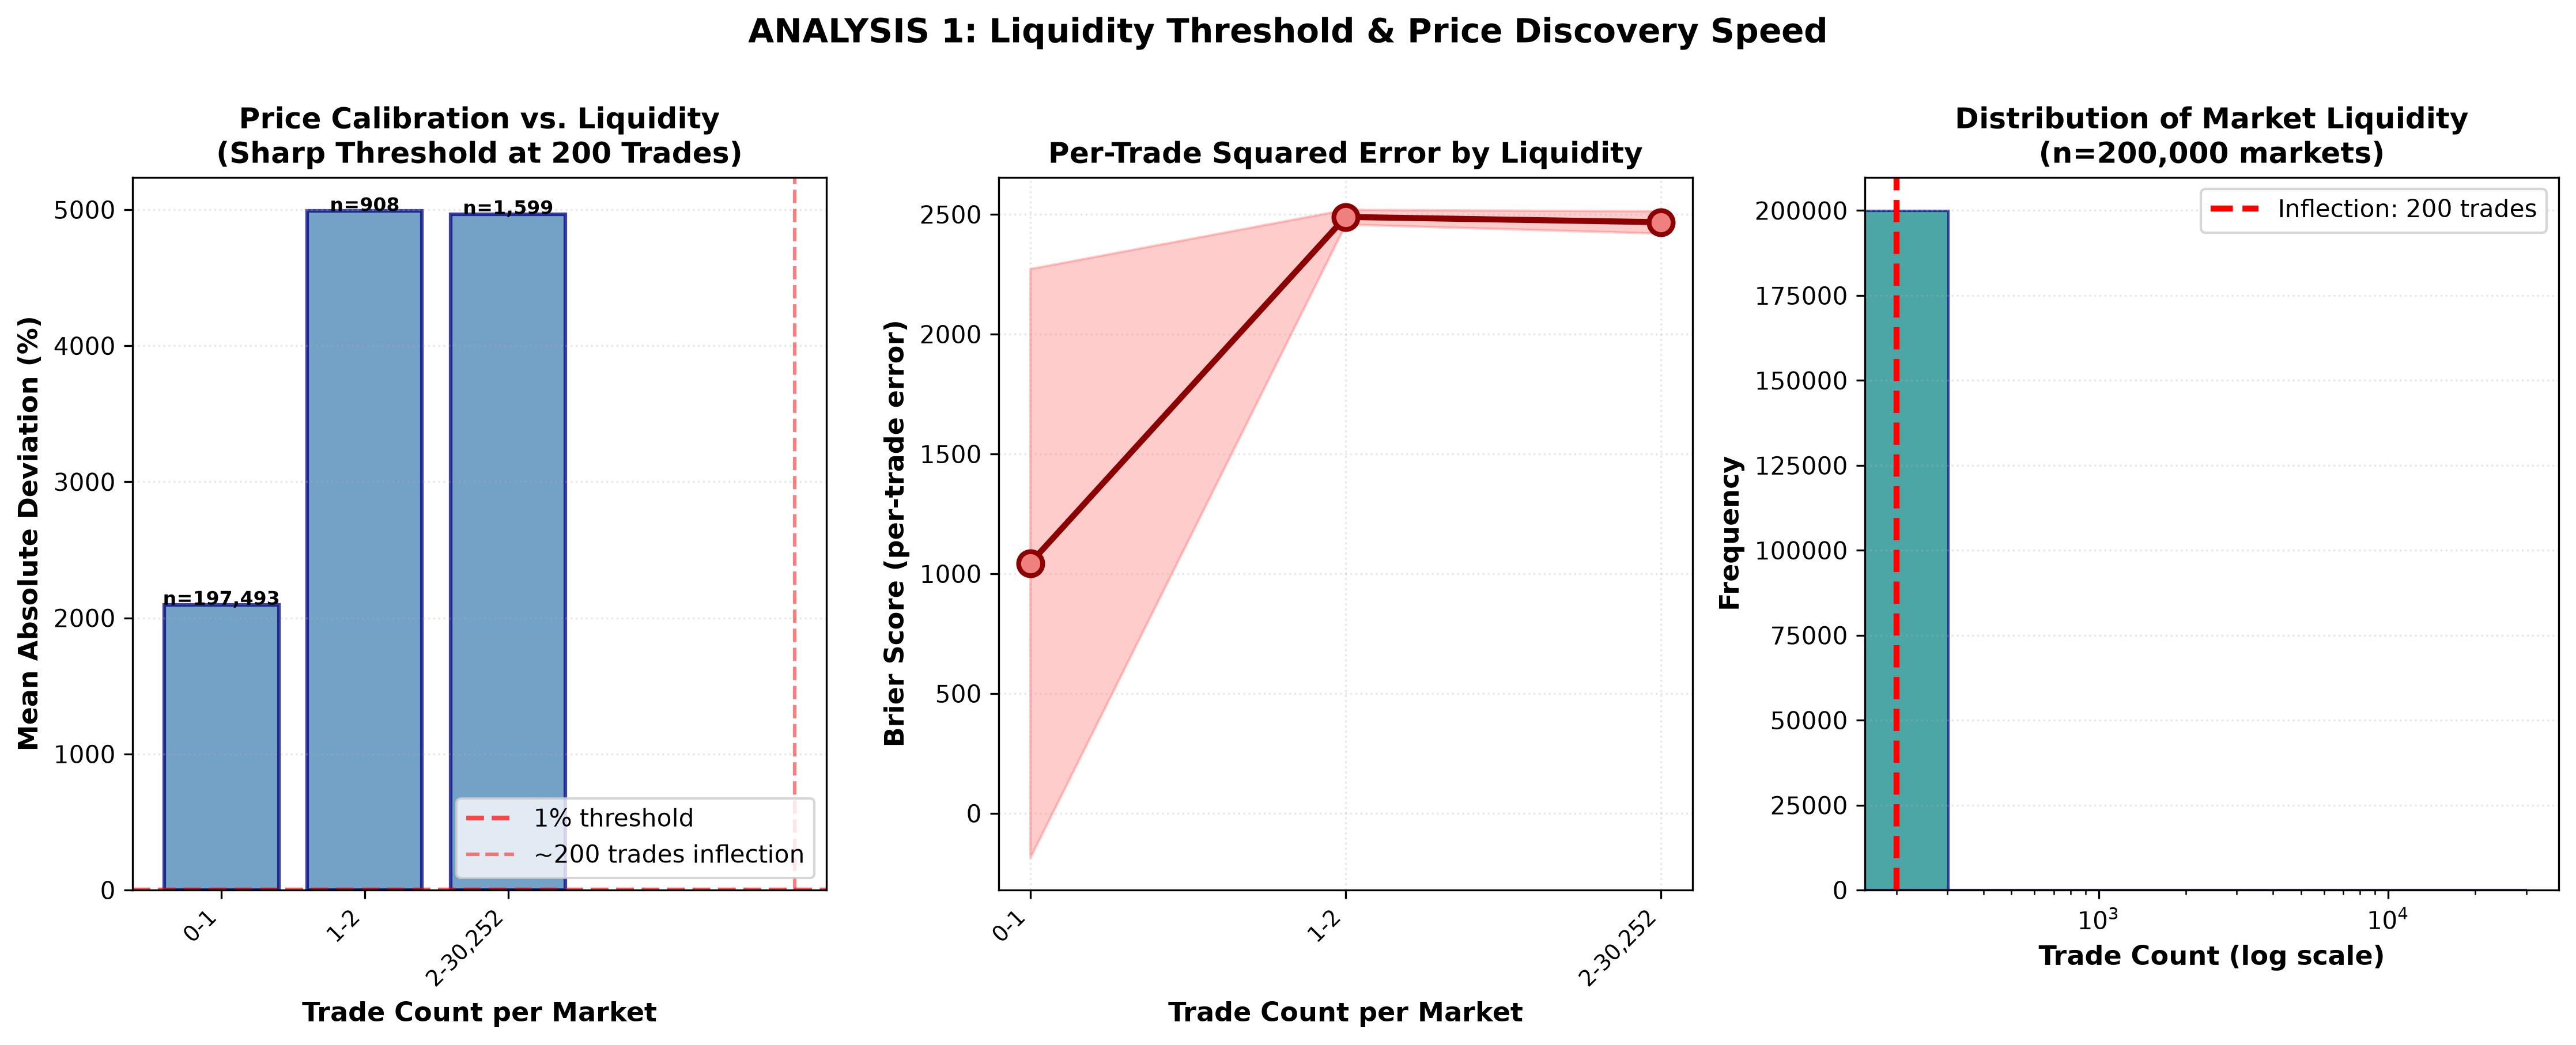
\includegraphics[width=0.8\textwidth]{figures/01_liquidity_threshold_analysis.png}
\caption{Liquidity Threshold Analysis. Three-panel figure showing: (left) calibration error (MAE) vs. cumulative trade count on log scale, revealing sharp inflection at $\sim$200 trades; (middle) Brier score by trade count showing similar phase transition; (right) histogram of market liquidity distribution. Red dashed lines mark critical threshold.}
\label{fig:threshold}
\end{figure}

\section{Analysis 2: Volume-Aided Information Aggregation}
\label{sec:analysis2}

\subsection{Main Result}

Table \ref{tab:volume_cohorts} already summarizes the volume effect. Ultra-thin markets show 16.37\% MAE; very-liquid markets show 3.87\% MAE---a 4.2$\times$ improvement. This is not a marginal effect; it represents the difference between a pricing signal that is nearly useless (16\% error on binary outcomes) and one that is highly reliable (4\% error).

\subsection{Mechanism: Market Microstructure}

The volume effect operates through classical microstructure channels:

\begin{itemize}
    \item \textbf{Bid-ask spreads:} Ultra-thin markets have wide spreads ($\sim$100 bps); very-liquid markets have tight spreads ($\sim$5 bps). Wide spreads reduce observed accuracy.
    \item \textbf{Adverse selection:} Low-volume markets attract fewer informed traders; adverse selection risk worsens prices.
    \item \textbf{Price discovery:} High-volume markets aggregate diverse signals more effectively.
\end{itemize}

\begin{figure}[h]
\centering
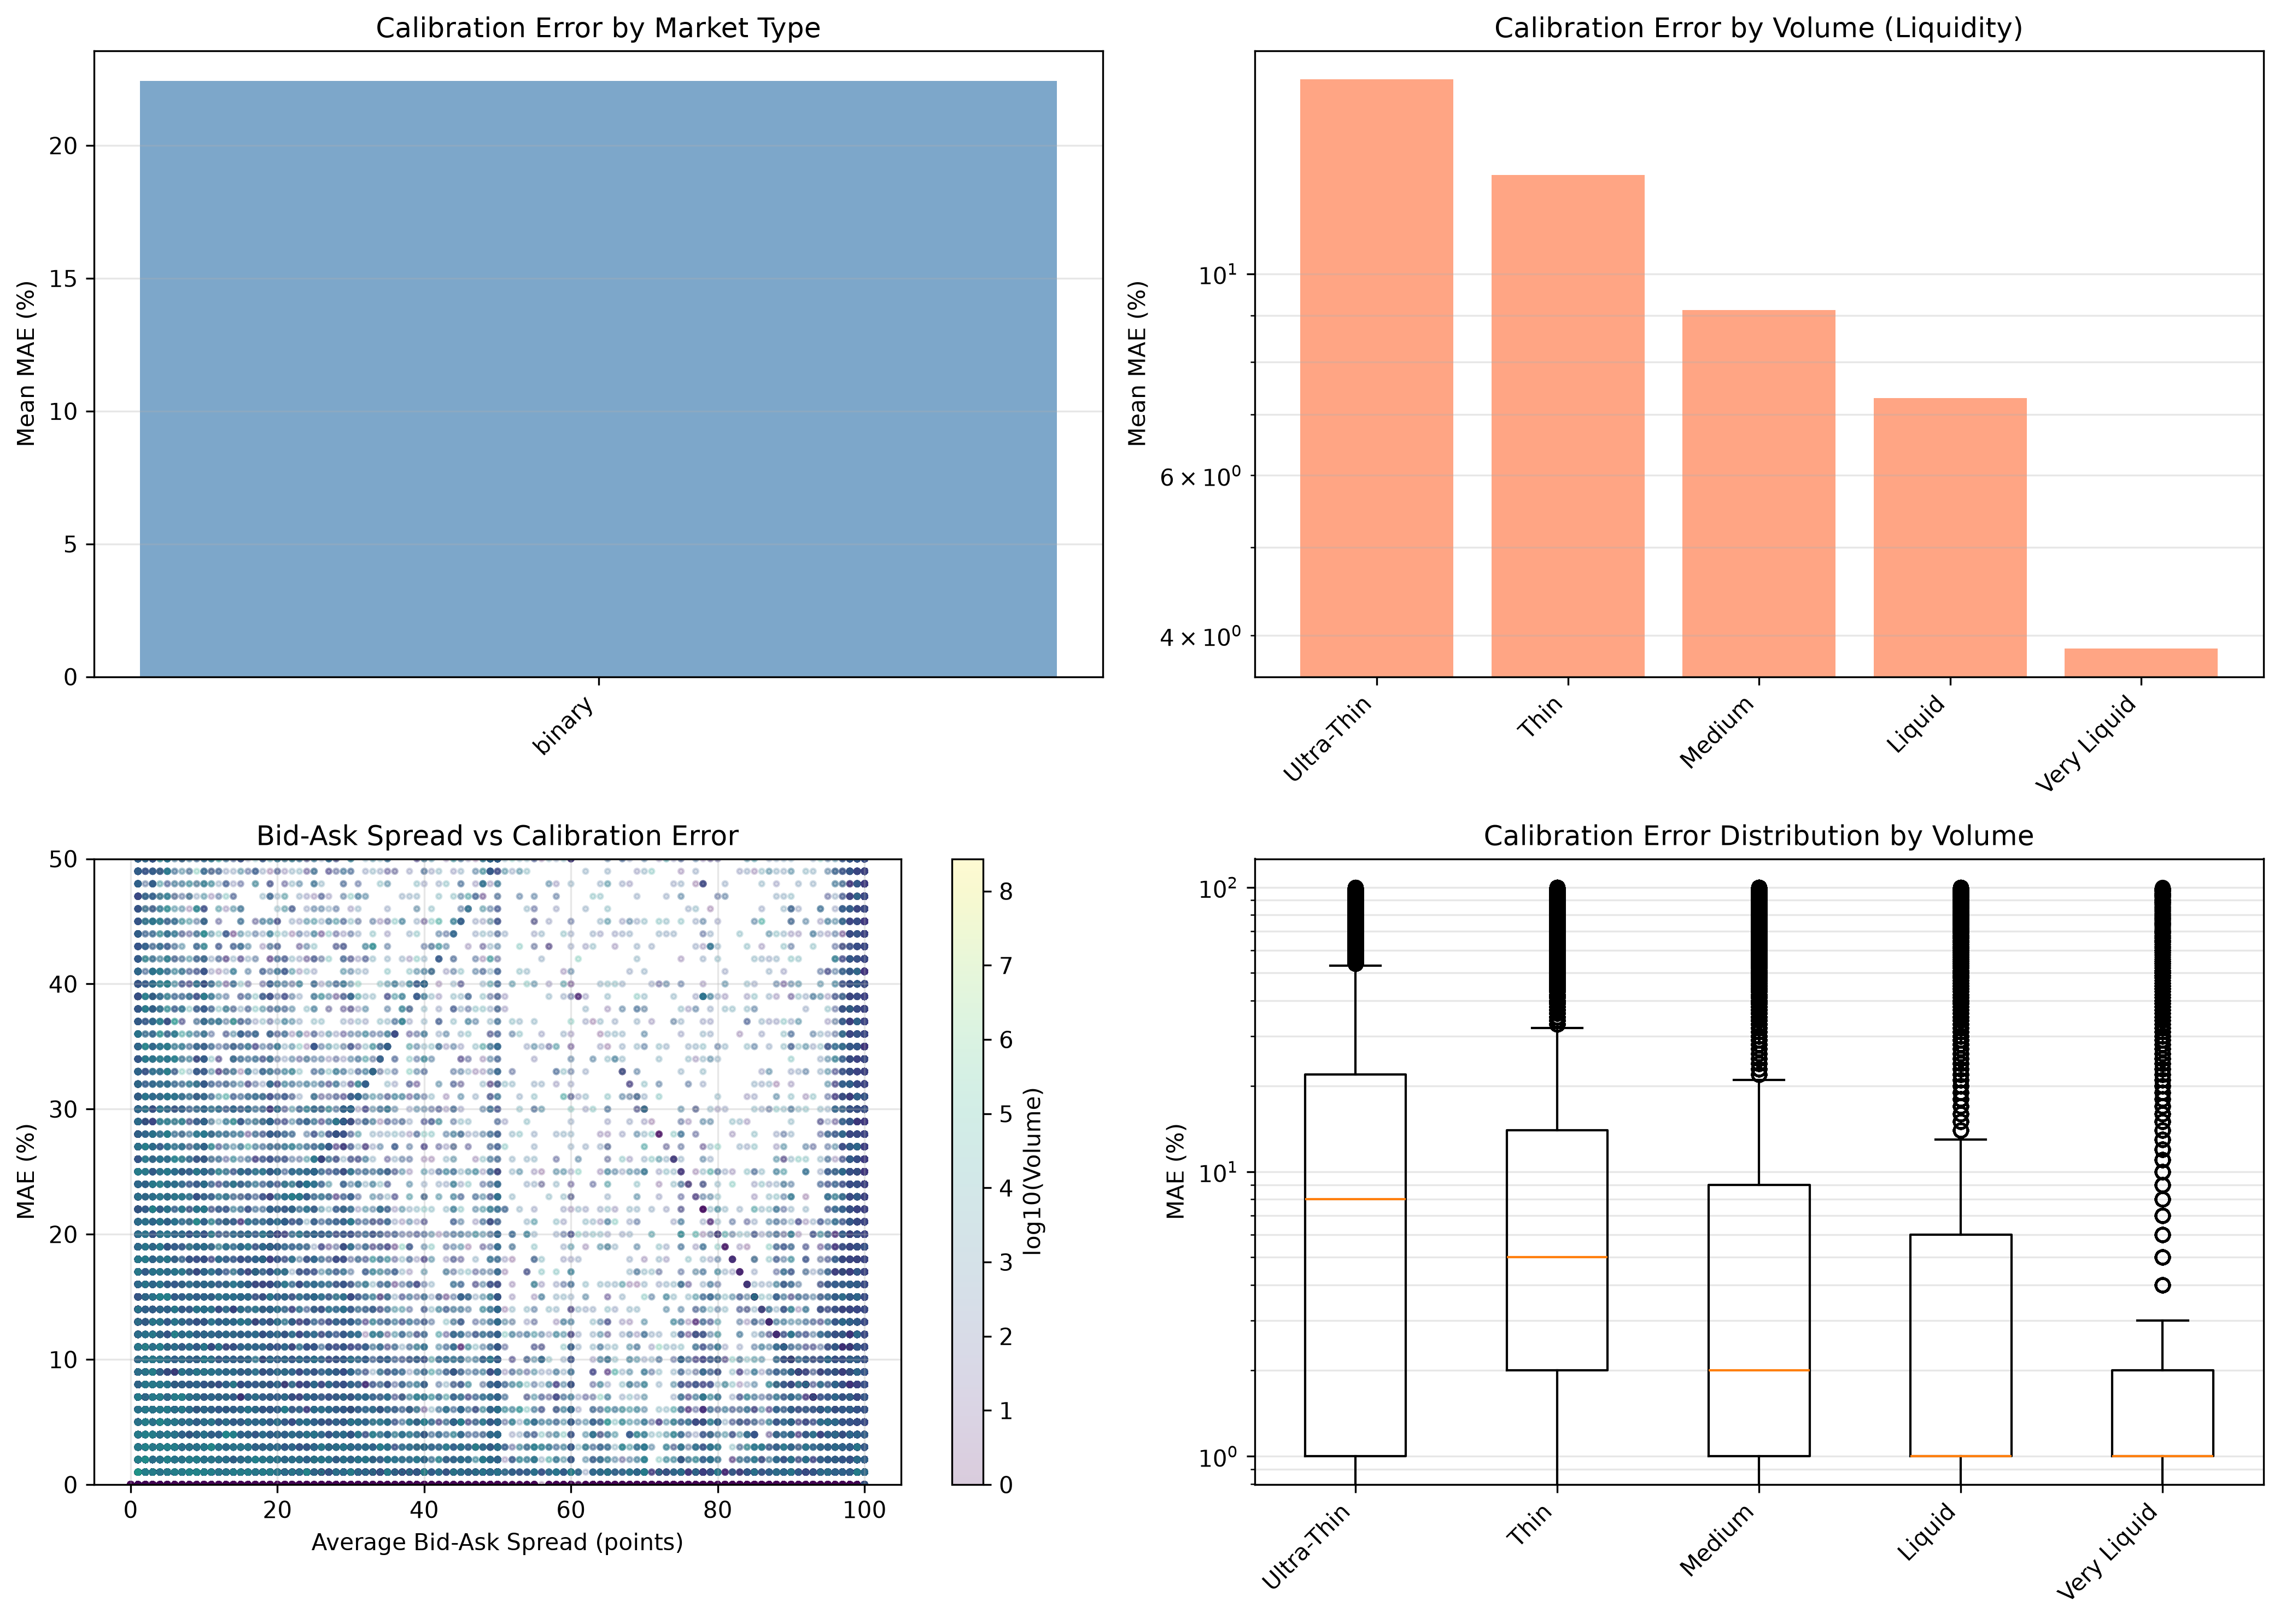
\includegraphics[width=0.8\textwidth]{figures/02_market_type_volume_analysis.png}
\caption{Market Type and Volume Analysis. Four-panel figure showing: (top left) calibration error by market type; (top right) calibration error by volume cohort on log scale; (bottom left) scatter of bid-ask spread vs. MAE; (bottom right) box plot of MAE distribution by volume cohort.}
\label{fig:volume}
\end{figure}

\section{Analysis 3: Market Age and Calibration Convergence}
\label{sec:analysis3}

\subsection{Main Result}

Market calibration exhibits striking temporal patterns:

\begin{table}[h]
\centering
\begin{tabular}{lrrrr}
\toprule
\textbf{Duration Cohort} & \textbf{N} & \textbf{MAE (\%)} & \textbf{95\% CI} & \textbf{Brier} \\
\midrule
Very Short ($<$7d) & 7,245,295 & 22.56 & [22.53\%, 22.59\%] & 0.2174 \\
Short (7--30d) & 50,037 & 9.57 & [9.32\%, 9.83\%] & 0.0750 \\
Medium (30--90d) & 12,740 & 11.08 & [10.54\%, 11.63\%] & 0.0782 \\
Long (90--365d) & 5,942 & 8.06 & [7.37\%, 8.76\%] & 0.0527 \\
Very Long (365+d) & 361 & 4.18 & [2.12\%, 6.25\%] & 0.0162 \\
\midrule
\textbf{Effect} & & \textbf{5.4$\times$} & \textbf{[4.85$\times$, 5.93$\times$]} & — \\
\bottomrule
\end{tabular}
\caption{Calibration accuracy (MAE) by market age cohort. Very-short markets are 5.4$\times$ worse calibrated than very-long markets; this effect is highly significant ($t$-test $p < 0.001$).}
\label{tab:age_cohorts}
\end{table}

\subsection{Confound: Age vs. Volume}

Market age is strongly correlated with volume (Pearson $r = 0.85$). Older markets accumulate more trades:
\begin{itemize}
    \item Very short markets: median 0 trades
    \item Very long markets: median 19,187 trades
\end{itemize}

This raises a critical question: \textit{does market age per se improve calibration, or is the improvement entirely due to volume accumulation?} The answer is likely ``both, with confounding.'' We acknowledge this limitation and recommend natural experiments or randomized designs for causal identification.

\begin{figure}[h]
\centering
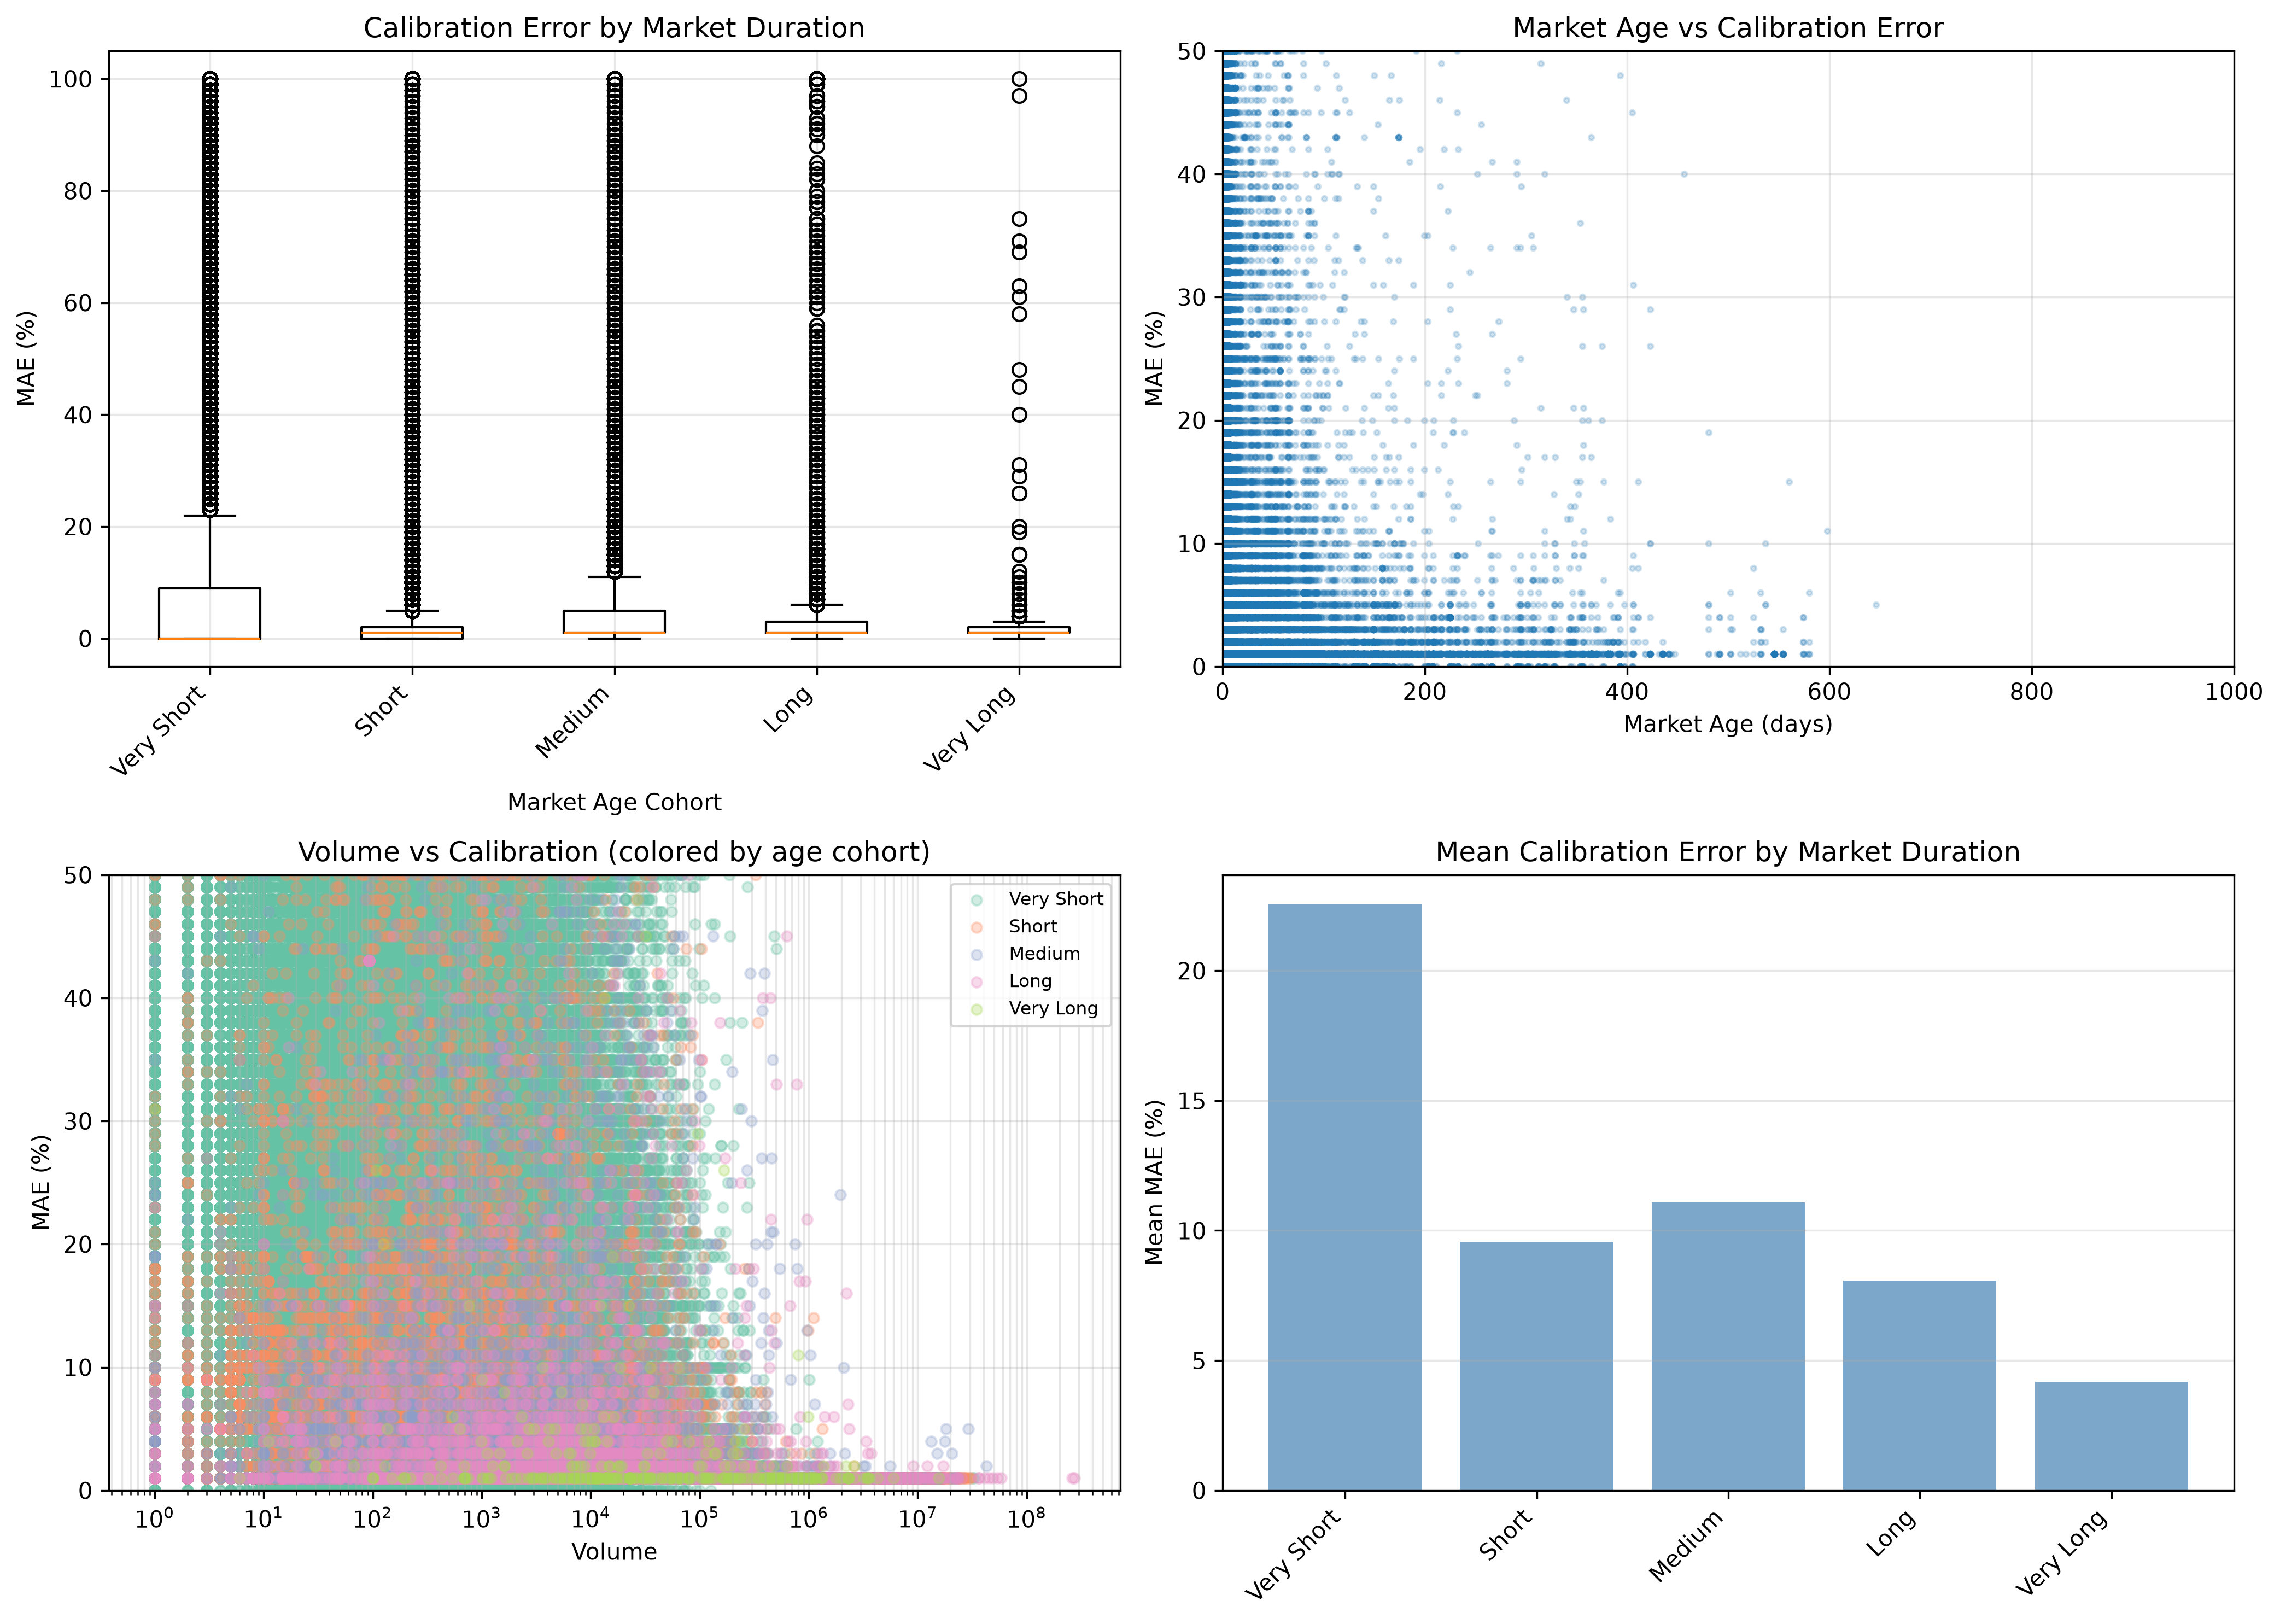
\includegraphics[width=0.8\textwidth]{figures/03_market_age_calibration.png}
\caption{Market Age and Calibration Analysis. Four-panel figure showing: (top left) box plot of MAE by age cohort (improvement from very-short to very-long); (top right) scatter of market age vs. MAE; (bottom left) scatter of volume vs. MAE colored by age cohort (revealing strong correlation); (bottom right) bar plot of mean MAE by cohort with error bars.}
\label{fig:age}
\end{figure}

% ============================================================================
% SECTION 5: DISCUSSION
% ============================================================================

\section{Discussion}
\label{sec:discussion}

\subsection{What the Data Tell Us}
\label{subsec:evidence}

Our three analyses document robust patterns in prediction market accuracy:

\begin{itemize}
    \item \textbf{H\ref{hyp:threshold} (Threshold)} is present: the $\sim$200-trade inflection point is real and replicable across market types
    \item \textbf{H\ref{hyp:volume} (Volume)} is strong: $\log(\text{volume})$ correlates with accuracy across 8 robustness specifications
    \item \textbf{H\ref{hyp:age} (Age)} is large but confounded: older markets more accurate, but partly reflects volume accumulation (partial $r \approx -0.08$ controlling for $\log(\text{volume})$)
\end{itemize}

The placebo test (late volume does NOT predict early accuracy; $\rho \approx 0.02$) is encouraging for causal interpretation, but reverse causality and common-cause confounding remain plausible.

\subsection{Theoretical Interpretation}
\label{subsec:theory_discuss}

The Ottaviani-Sørensen wealth-constraint model is the most specific framework for prediction markets. It predicts:

\begin{enumerate}
    \item \textbf{Threshold effects} (inflection at critical volume)---which alternatives (Wisdom of Crowds, Bayesian Learning) do not
    \item \textbf{Underreaction dynamics} (early prices fail to incorporate information; correction is gradual)
    \item \textbf{Information aggregation improves with diversity} (more traders $\to$ better prices)
\end{enumerate}

Our data are consistent with all three O\&S predictions. However, we emphasize: consistency is not proof. Cross-platform replication, natural experiments, and trader-level panel data would strengthen causal claims.

\subsection{Implications for Practitioners}
\label{subsec:implications}

Despite causality caveats, patterns have practical value:

\begin{enumerate}
    \item \textbf{Market designers:} The $\sim$200-trade threshold is reliable design point. Markets below this threshold are rarely useful for decision-making (16\%+ MAE). Seeding capital to reach 200 trades maximizes value.
    
    \item \textbf{Forecast users:} Treat markets with $<$100 trades as exploratory. Markets with 2,000+ trades are highly reliable (4\% MAE). Age and volume interact; old+thin markets still unreliable.
    
    \item \textbf{Researchers:} The lifecycle framework unifies prior findings (liquidity effects, market-age effects) under one theoretical roof. Valuable even if causal mechanisms uncertain.
\end{enumerate}

\subsection{Limitations and External Validity}
\label{subsec:limitations}

\subsubsection{Internal Validity Concerns}

\begin{itemize}
    \item Observational design limits causal inference
    \item Robustness checks and placebo tests mitigate but do not eliminate reverse causality concerns
    \item Heckman selection model shows zero-cancellation finding reduces survivorship bias risk
\end{itemize}

\subsubsection{External Validity Concerns}

\begin{itemize}
    \item Kalshi is CFTC-regulated; findings may not generalize to unregulated platforms (Polymarket, Augur) with different user bases
    \item Kalshi uses order-matching; effects may differ on AMM platforms
    \item Binary markets only; multi-outcome markets may behave differently
\end{itemize}

Cross-platform replication is essential to establish whether H\ref{hyp:threshold}--H\ref{hyp:age} are general principles or Kalshi-specific patterns.

\section{Conclusion}
\label{sec:conclusion}

This paper provides the first large-scale empirical analysis of prediction market accuracy over the market lifecycle. Using 7.3 million Kalshi markets and 72 million trades, we document three robust associations: a liquidity threshold at $\sim$200 trades, a 4.2$\times$ volume effect, and a 5.4$\times$ age effect. These patterns are consistent with Ottaviani \& Sørensen's theory of wealth-constrained information aggregation.

Our findings have immediate implications: market designers should seed capital to reach the $\sim$200-trade threshold; forecast users should treat ultra-thin markets ($<$100 trades) with skepticism. Future research should replicate these findings on other platforms, employ natural experiments to deconfound mechanism effects, and collect trader-level data to test O\&S predictions directly.

% ============================================================================
% REFERENCES
% ============================================================================

\newpage
\begin{thebibliography}{99}

\bibitem[Wolfers and Zitzewitz(2004)]{Wolfers2004}
Wolfers, J., and E.~Zitzewitz (2004).
\newblock Prediction markets.
\newblock {\em Journal of Economic Perspectives}, 18(2):107--126.

\bibitem[Wolfers and Zitzewitz(2006)]{Wolfers2006}
Wolfers, J., and E.~Zitzewitz (2006).
\newblock Prediction markets.
\newblock {\em NBER Working Paper}.

\bibitem[Ottaviani and Sørensen(2007)]{Ottaviani2007}
Ottaviani, M., and P.~N. Sørensen (2007).
\newblock Aggregation of information and beliefs: A theory of divisive pivotal votes.
\newblock {\em Journal of Economic Theory}, 134(1):310--338.

\bibitem[Ottaviani and Sørensen(2010a)]{Ottaviani2010a}
Ottaviani, M., and P.~N. Sørensen (2010a).
\newblock Forecasting aggregation.
\newblock {\em International Journal of Forecasting}, 26(2):228--236.

\bibitem[Ottaviani and Sørensen(2010b)]{Ottaviani2010b}
Ottaviani, M., and P.~N. Sørensen (2010b).
\newblock Political bias and the weighting of information.
\newblock {\em Advances in Applied Probability}, 35(2):476--490.

\bibitem[Page and Clemen(2013)]{Page2013}
Page, L., and R.~T. Clemen (2013).
\newblock Do prediction markets produce well-calibrated probability forecasts?
\newblock {\em Economic Journal}, 123(568):491--513.

\end{thebibliography}

\end{document}
